% !TeX root = ../main.tex
% Add the above to each chapter to make compiling the PDF easier in some editors.

\chapter{Variational Autoencoder}\label{chapter:vae}

In Section \ref{sec:cs_with_gen}, we explored how generative models can be used to solve compressed sensing tasks.
These models allow for transforming high-dimensional data into more manageable, compressed representations.
Among the different types of generative models, the \gls{VAE} \parencite{VAE} is chosen for this thesis, as outlined in Section \ref{subsec:gen_models}.
Though improved variants of the \gls{VAE} exist, such as the $\beta$-\gls{VAE} \parencite{Beta-VAE},  this thesis focuses on the original \gls{VAE} by \textcite{VAE}, due to its simplicity.
The following sections will explore the architecture of the \gls{VAE} implemented, along with the fine-tuning strategy for improving reconstruction quality in the case study cities.

\section{Training}
\gls{VAE}s consist of an encoder and a decoder that are typically symmetrical in architecture \parencite{VAE}.
The encoder is a neural network that outputs a distribution in terms of a mean and the logarithm of a variance in the latent space given an emission field as input. The decoder outputs an emission field from a variable sampled from the latent space.

\gls{VAE}s are trained to fulfill two main objectives \parencite{VAE}.
First, any input sample emission field run through the encoder and decoder end-to-end is reconstructed as accurately as possible.
The \gls{MSE} between the input and the reconstructed output is minimized for this.
Second, the encoder outputs a distribution as close as possible to a standard Gaussian distribution $\mathcal{N}(0, I)$.
To achieve this, the \gls{KL} divergence between the encoder's output distribution and the standard normal distribution is minimized.
A reparameterization trick is employed during training to deal with the randomness in the encoder output \parencite{VAE}.
The loss is then a combination of both objectives:
\begin{equation}
    L(x, \hat{x}) = \frac{1}{N}\sum_{i=1}^N \norm{x_i - \hat{x}_i}_2^2 + D_{\text{\gls{KL}}}(q(z|x) \rVert p(z))
\end{equation}
where $x$ is the input emission field, $\hat{x}$ is the reconstructed emission field, $q(z|x)$ is the encoder's output distribution, $p(z)$ is the prior distribution (standard normal), and $D_{\text{\gls{KL}}}$ is the \gls{KL} divergence.
Minimizing this loss is equivalent to maximizing the \gls{ELBO}.

Besides the loss, at each step, the structural similarity of reconstructions is investigated by computing the \gls{SSIM}.

\section{Architecture Search} \label{section:architecture_search}
Searching for optimal hyperparameters is challenging with many different approaches \parencite{HyperParameters}.
In particular, designing a good architecture takes a lot of trial and error.
Thus, different architectures are explored to determine a suitable one.
For this, a baseline architecture is first established.
Then, different variations of this architecture are explored and trained.
The model's architecture with the best performance is then chosen as the model architecture for this thesis.

Each variation is trained for $20$ epochs on the data from $2015$ only.
The dataset split is $t=0.15$, $v=0.15$, with the test set not being used.
The batch size is $32$.
The optimizer AmsGrad \parencite{AmsGrad} is used with a learning rate of $10^{-3}$.
Gradients are clipped at $0.5$.

\subsection{Baseline Architecture}
The baseline architecture is inspired by the work by \textcite{Tightrope}.
This means that the bottleneck layers have a high width and height.
As the input width and height of the emission fields are $32$ by $32$, the bottleneck width and height are chosen as $8$ by $8$.
Inspired by \textcite{AllConvolutional}, to reduce the width and height dimensions, instead of using pooling operations, two strided convolutions are used.
The strided convolutions, depicted in Figure \ref{fig:conv_layer}, have kernel size $2$ and stride $2$, thus halving the size.

\begin{figure}[htb]
    \centering
    \begin{subfigure}[b]{0.45\textwidth}
        \centering
        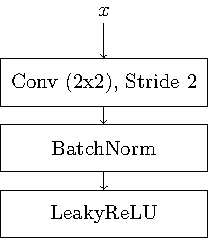
\includegraphics[]{figures/model_architecture/build/conv_layer.pdf}
        \caption{Conv Layer}
        \label{fig:conv_layer}
    \end{subfigure}
    \hfill
    \begin{subfigure}[b]{0.45\textwidth}
        \centering
        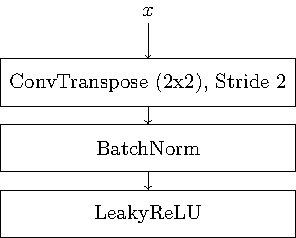
\includegraphics[]{figures/model_architecture/build/deconv_layer.pdf}
        \caption{DeConv Layer}
        \label{fig:deconv_layer}
    \end{subfigure}
    \caption{Composition of Strided Convolution Layers in VAE}
    \label{fig:strided_convolutions}
\end{figure}

The strided convolution layers make use of the LeakyReLU activation function and batch normalization \parencite{BatchNorm} as a regularization technique.
Conversely, in the decoder, two strided transpose convolutions, depicted in Figure \ref{fig:deconv_layer}, with the same parameters, are used to double the width and height instead of upsampling layers.

In between the strided convolutions, \gls{ResConv} \parencite{ResNet} are used.
They can be seen in Figure \ref{fig:resconv}.
\begin{figure}[htb]
    \centering
    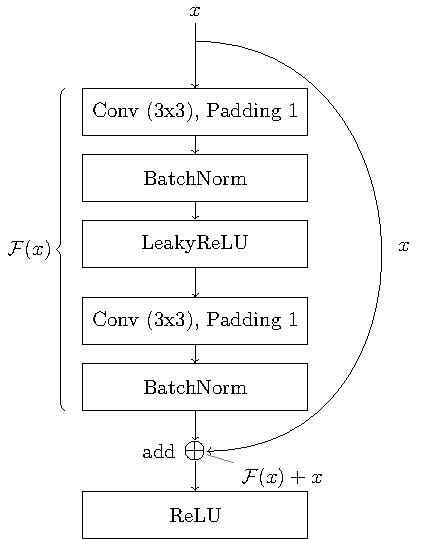
\includegraphics[]{figures/model_architecture/build/residual_conv_layer.pdf}
    \caption{Composition of ResConv Layer in VAE \parencite{ResNet}}
    \label{fig:resconv}
\end{figure}
The \gls{ResConv} layers use two convolutions with kernel size $3$ and padding $1$ to retain the width and height dimensions.
The output activation is ReLU.
In between the two convolutional layers, LeakyReLU is used again.
Batch normalization is applied after each convolution.

\begin{figure}[htb]
    \centering
    \begin{minipage}[b]{\textwidth}
        \centering
        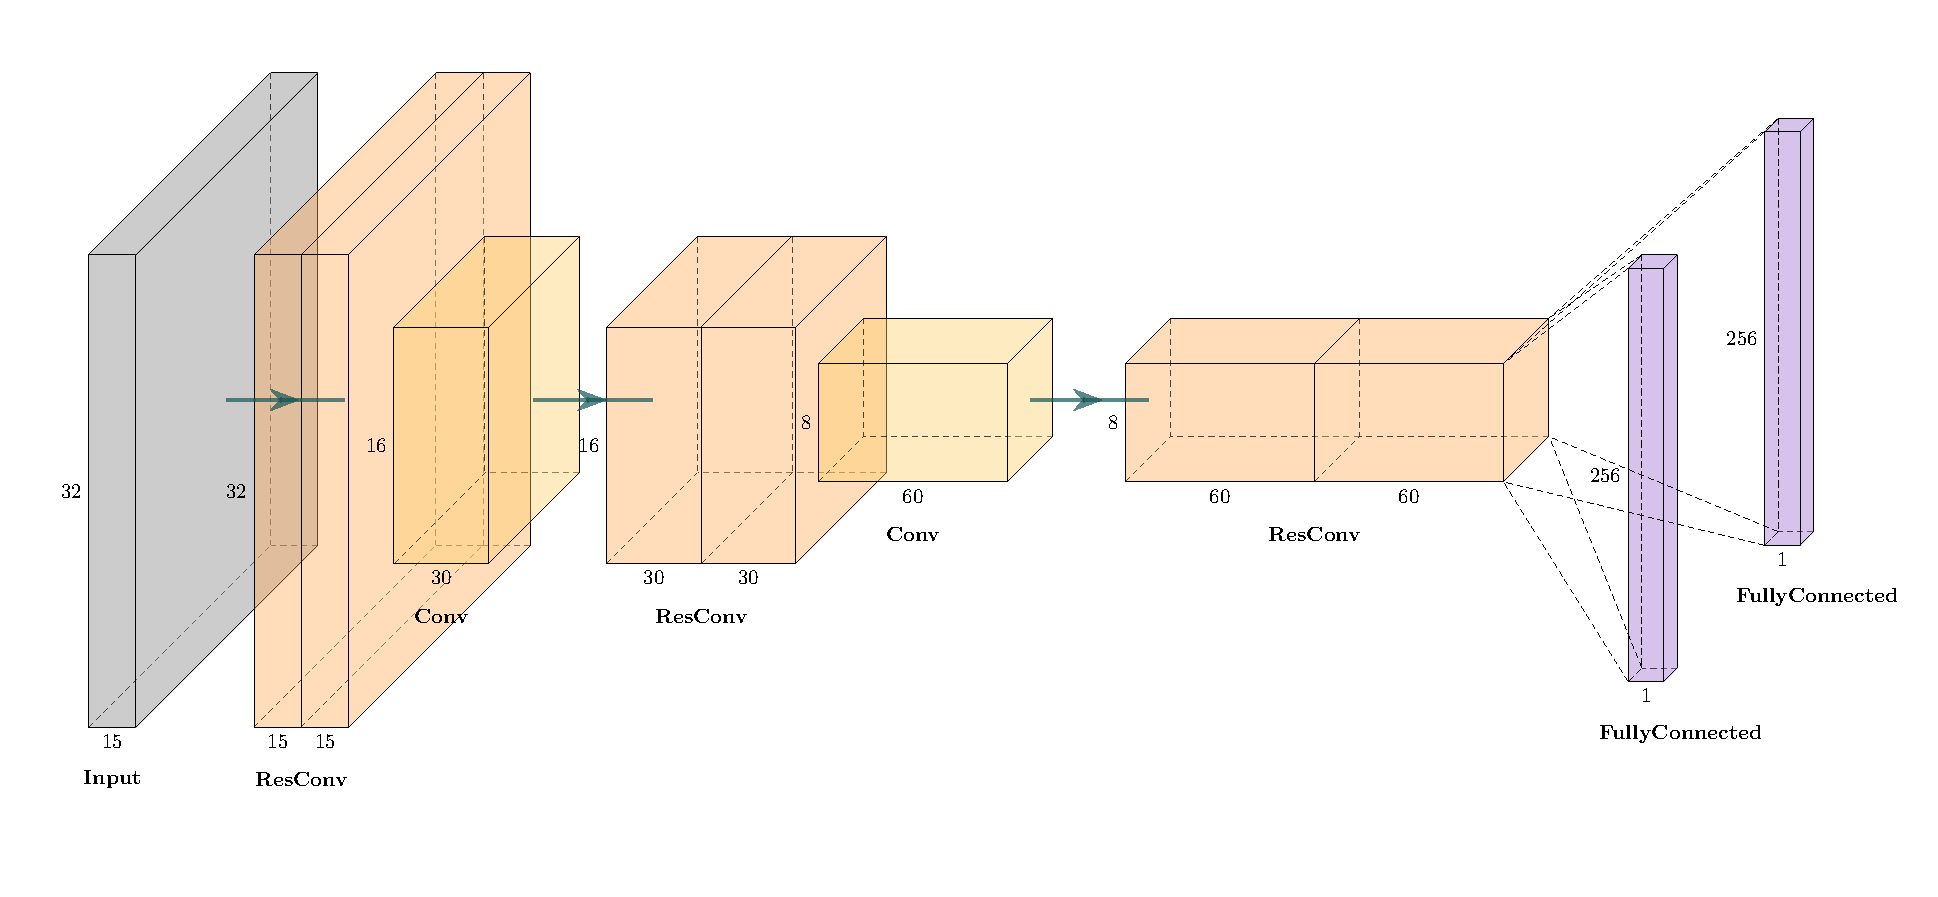
\includegraphics[width=\textwidth]{figures/model_architecture/build/baseline_vae_encoder.pdf}
        \caption{Baseline VAE Encoder Architecture (generated with \parencite{NNVisualization})}
        \label{fig:baseline_encoder}
    \end{minipage}
    \begin{minipage}[b]{\textwidth}
        \centering
        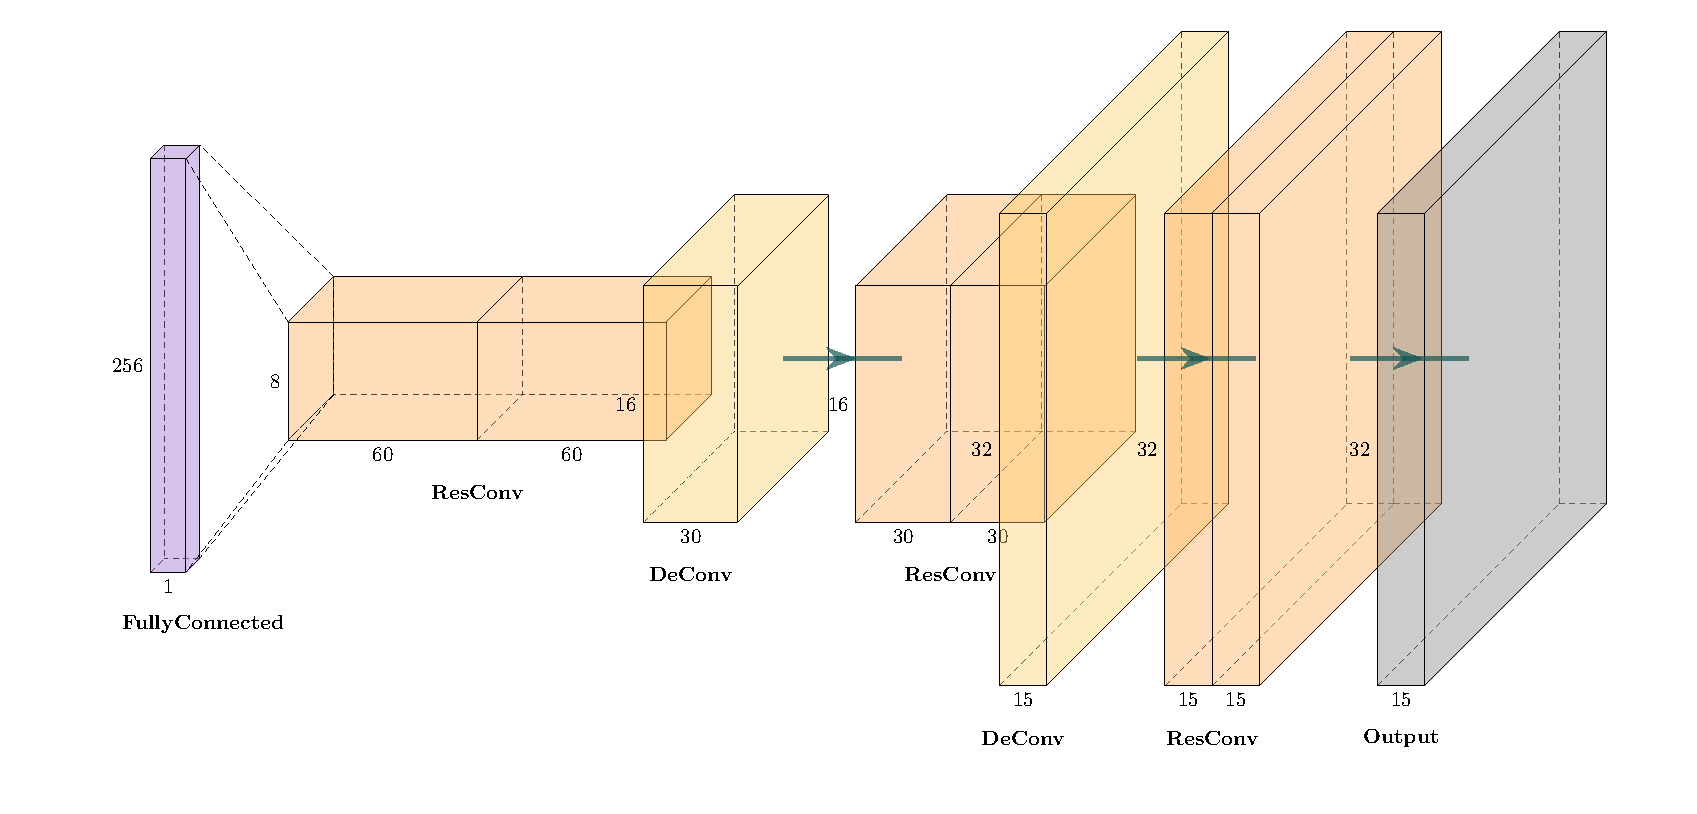
\includegraphics[width=\textwidth]{figures/model_architecture/build/baseline_vae_decoder.pdf}
        \caption{Baseline VAE Decoder Architecture (generated with \parencite{NNVisualization})}
        \label{fig:baseline_decoder}
    \end{minipage}
\end{figure}

Figures \ref{fig:baseline_encoder} and \ref{fig:baseline_decoder} show the baseline encoder and decoder architectures, respectively.
In both the encoder and decoder, the two strided convolutions are located after two layers of \gls{ResConv} layers each.
At the end of the encoder, two fully connected layers are used to output the mean and logarithmic variance of the latent space with a dimension of $256$.
Conversely, at the input of the decoder, a fully connected layer transforms the $256$-dimensional latent vector into the size of the first bottleneck layer.
Finally, it should be noted that the last \gls{ResConv} layer in the decoder does not use batch normalization.

\subsection{Explored Variations}
The following architectural variations were explored to improve the baseline model: 
\begin{enumerate}
    \item \textbf{Convolutional layers with pooling and upsampling}: This variation increased or decreased the depth using convolutional layers, while pooling layers were used to reduce width and height, and upsampling layers were employed to increase the width and height in the decoder.
    \item \textbf{Upsampling emission fields to 64x64}: The emission fields were upsampled to $64 \times 64$, and then convolutions were applied. In the decoder, max pooling was used to downsample the resolution back to $32 \times 32$.
    \item \textbf{Increased depth}: Instead of simply doubling the depth, this variation quadrupled the depth, aiming to capture more complex features.
    \item \textbf{Two convolutional layers for dimension changes}: This variation replaced the strided convolution used to reduce or increase the dimensions with two convolutional layers for the same task, offering potentially finer control over the dimensionality change. 
    \item \textbf{Three \gls{ResConv} layers}: Here, the number of \gls{ResConv} was increased to three, enhancing the model’s depth and capacity to learn more intricate patterns.
    \item \textbf{Residual layers with identity mappings}: Inspired by \parencite{IdentityMappings}, the \gls{ResConv} layers were replaced with residual layers that incorporated identity mappings to improve feature propagation across layers, as seen in Figure \ref{fig:identity_mappings}.
    \item \textbf{Residual layers with identity mappings and dropout}: Based on \parencite{WideResNet}, dropout was added to the residual layers with identity mappings to reduce overfitting and improve generalization.
\end{enumerate}

\begin{figure}[htb]
    \centering
    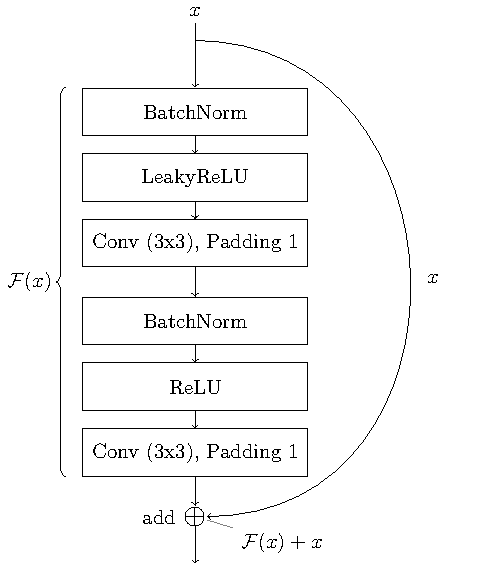
\includegraphics[]{figures/model_architecture/build/residual_conv_with_im_layer.pdf}
    \caption{Composition of ResConv Layer With Identity Mappings in VAE \parencite{IdentityMappings}}
    \label{fig:identity_mappings}
\end{figure}

The performance of these variations was evaluated over 20 training epochs.
Figure \ref{fig:validation_losses} presents the validation loss for each variation, while Figure \ref{fig:validation_ssim} shows the corresponding validation \gls{SSIM}.
These metrics help determine which variations provided improvements over the baseline architecture.

\begin{figure}
    \centering
    \begin{subfigure}{0.49\textwidth}
        \centering
        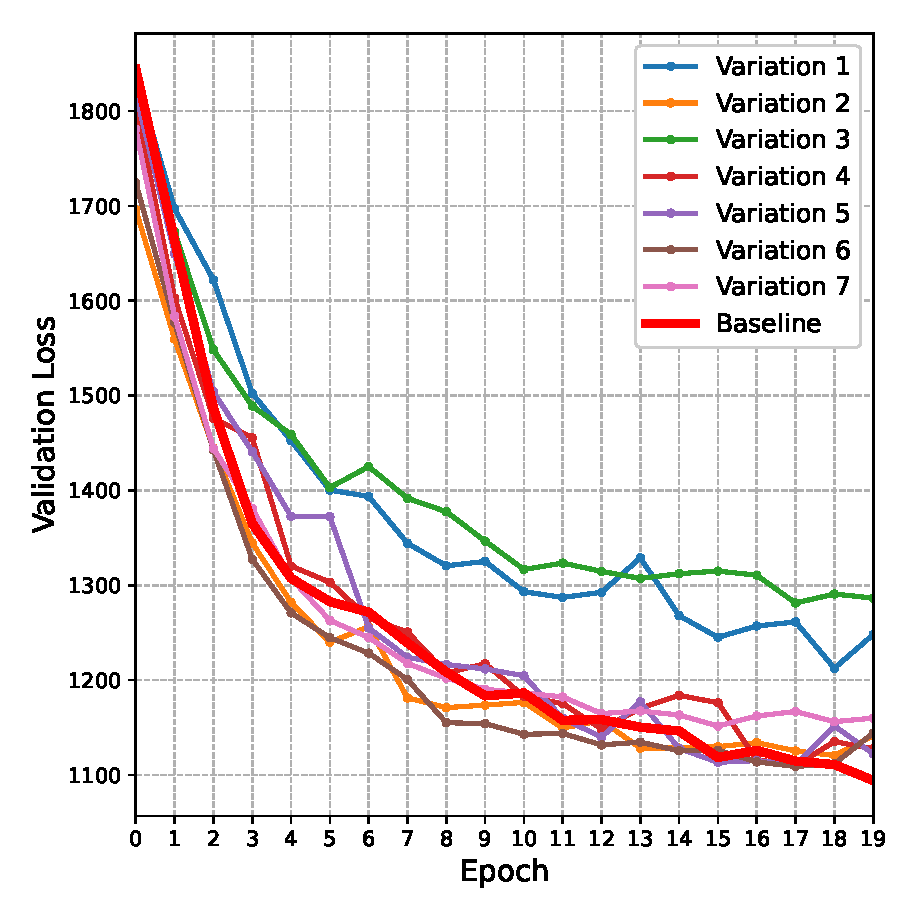
\includegraphics[width=\linewidth]{figures/architecture_search/architecture_search_loss.eps}
        \caption{Validation Loss}
        \label{fig:validation_losses}
    \end{subfigure}%
    \begin{subfigure}{0.49\textwidth}
        \centering
        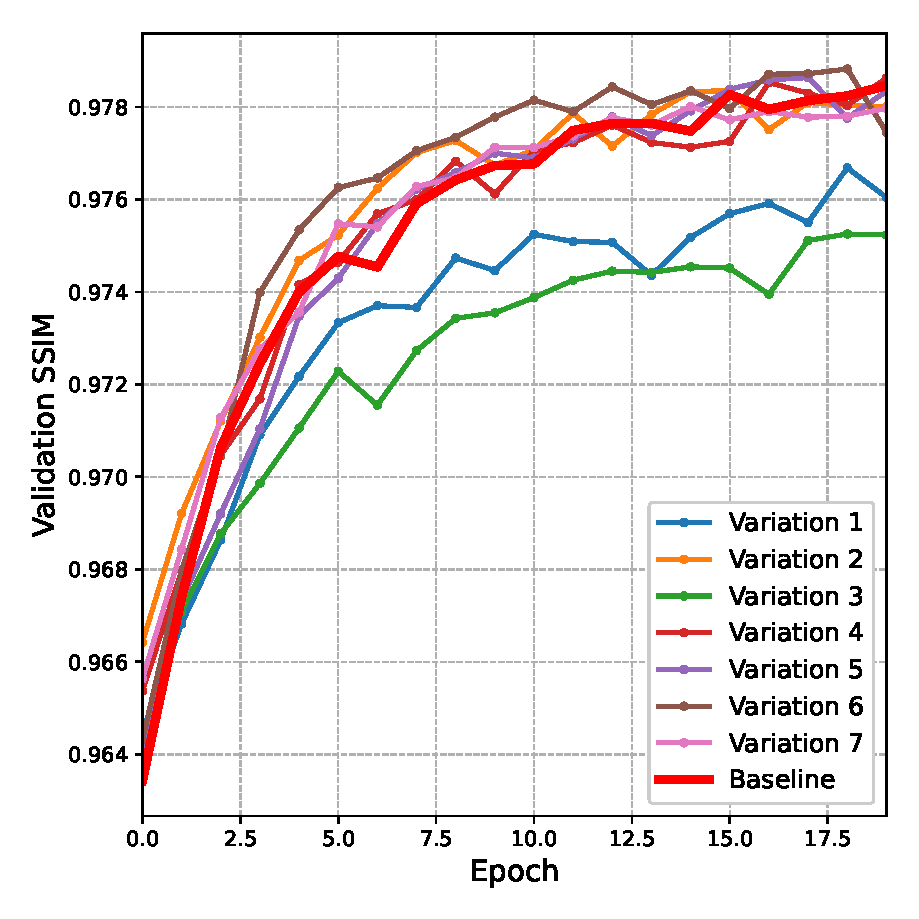
\includegraphics[width=\linewidth]{figures/architecture_search/architecture_search_ssim.eps}
        \caption{Validation SSIM}
        \label{fig:validation_ssim}
    \end{subfigure}
    \caption{Validation Loss and SSIM of Variations During Training in Architecture Search}
    \label{fig:test}
\end{figure}

The results reveal that the baseline architecture performs consistently well in both validation loss and \gls{SSIM}, providing a solid foundation.
Among the variations, Variation 6 (Identity Mapping) performs the best in terms of \gls{SSIM}, indicating that identity mappings significantly enhance the model’s ability to preserve structure and detail.
Variation 7 (Identity Mappings with Dropout) closely follows, with dropout helping to mitigate overfitting, particularly for larger datasets.

Conversely, Variation 3, which increased the model’s depth, struggled to match the performance of the baseline, suggesting that simply increasing depth can lead to over-parameterization and vanishing gradients without additional architectural changes.
Other variations provided no improvements or even decreased performance, like Variation 1. 

\subsection{Final Architecture} \label{subsection:final_architecture}
Based on these insights, the final architecture incorporates identity mappings and dropout, as proposed in Variation 7, and increases the number of residual layers to three, as seen in Variation 5.
These changes provide a balanced approach to improving generalization, reducing overfitting, and preserving high-quality reconstructions.
The final encoder and decoder architectures can be seen in Figure \ref{fig:final_encoder} and Figure \ref{fig:final_decoder}.

\begin{figure}[htb]
    \centering
    \begin{minipage}[b]{\textwidth}
        \centering
        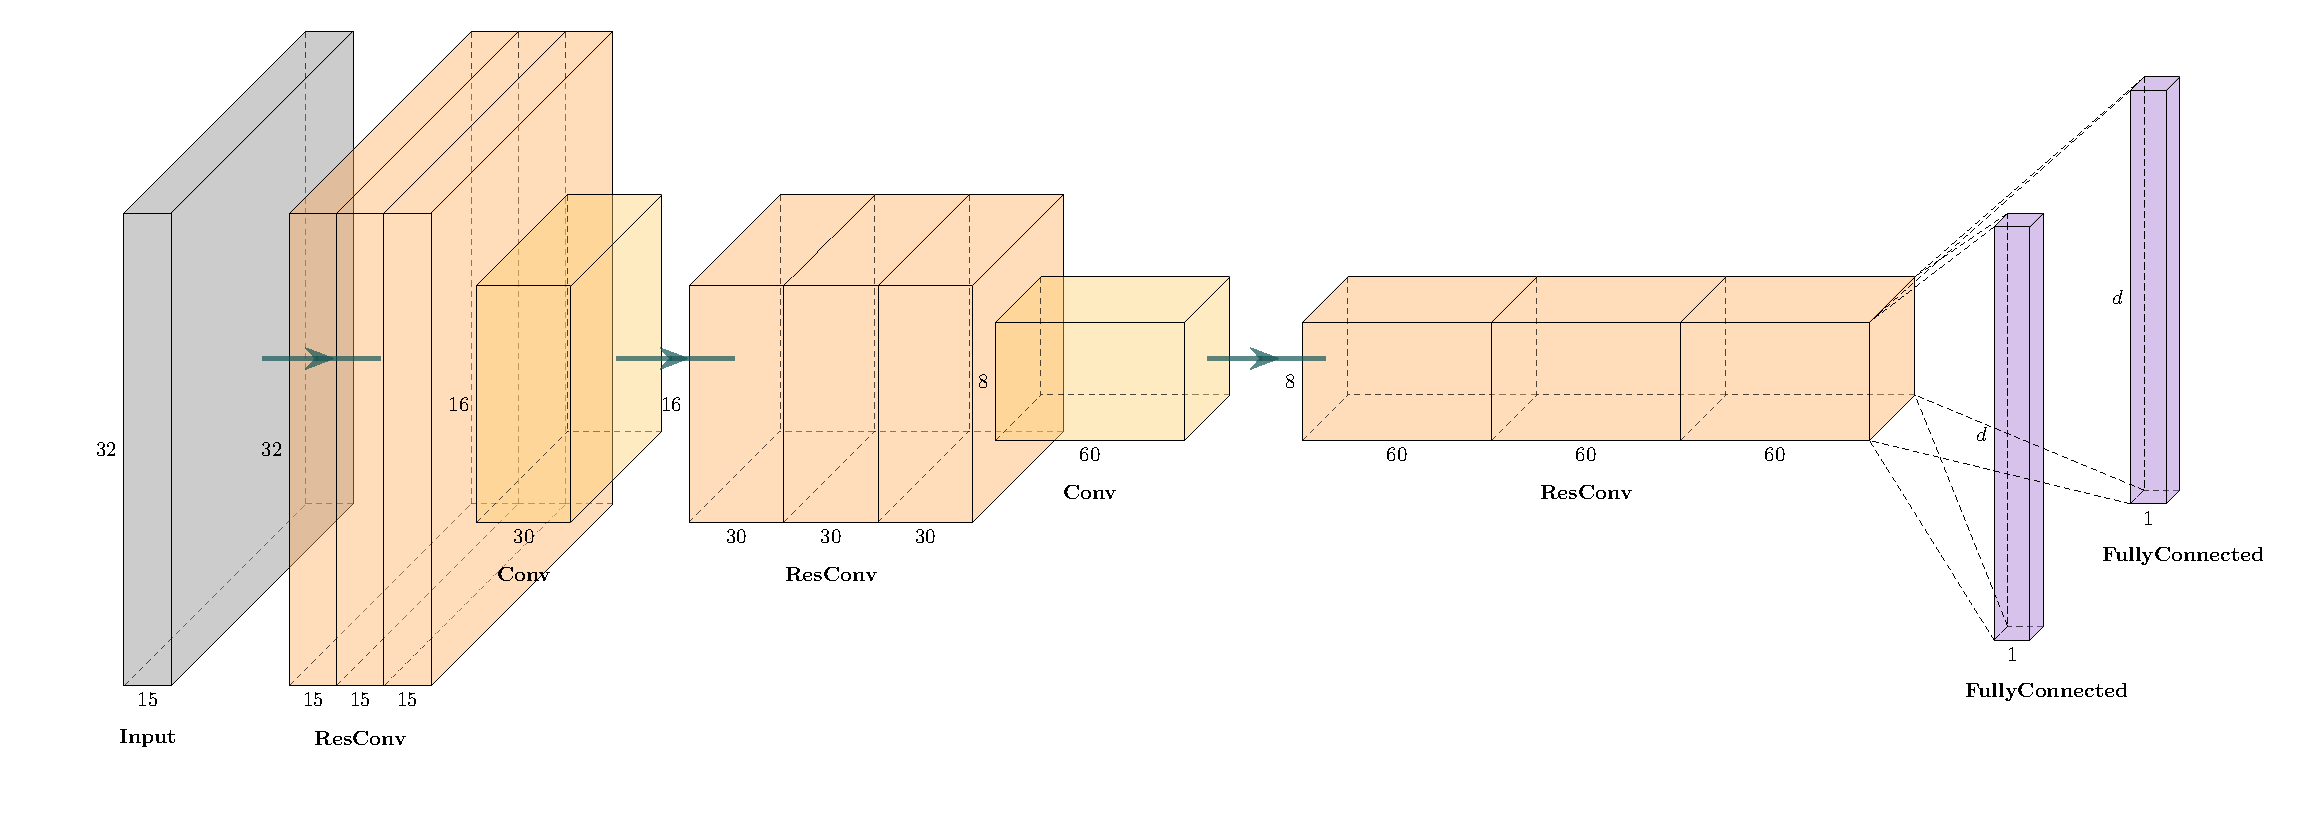
\includegraphics[width=\textwidth]{figures/model_architecture/build/final_vae_encoder.pdf}
        \caption{Final VAE Encoder Architecture (generated with \parencite{NNVisualization})}
        \label{fig:final_encoder}
    \end{minipage}
    \begin{minipage}[b]{\textwidth}
        \centering
        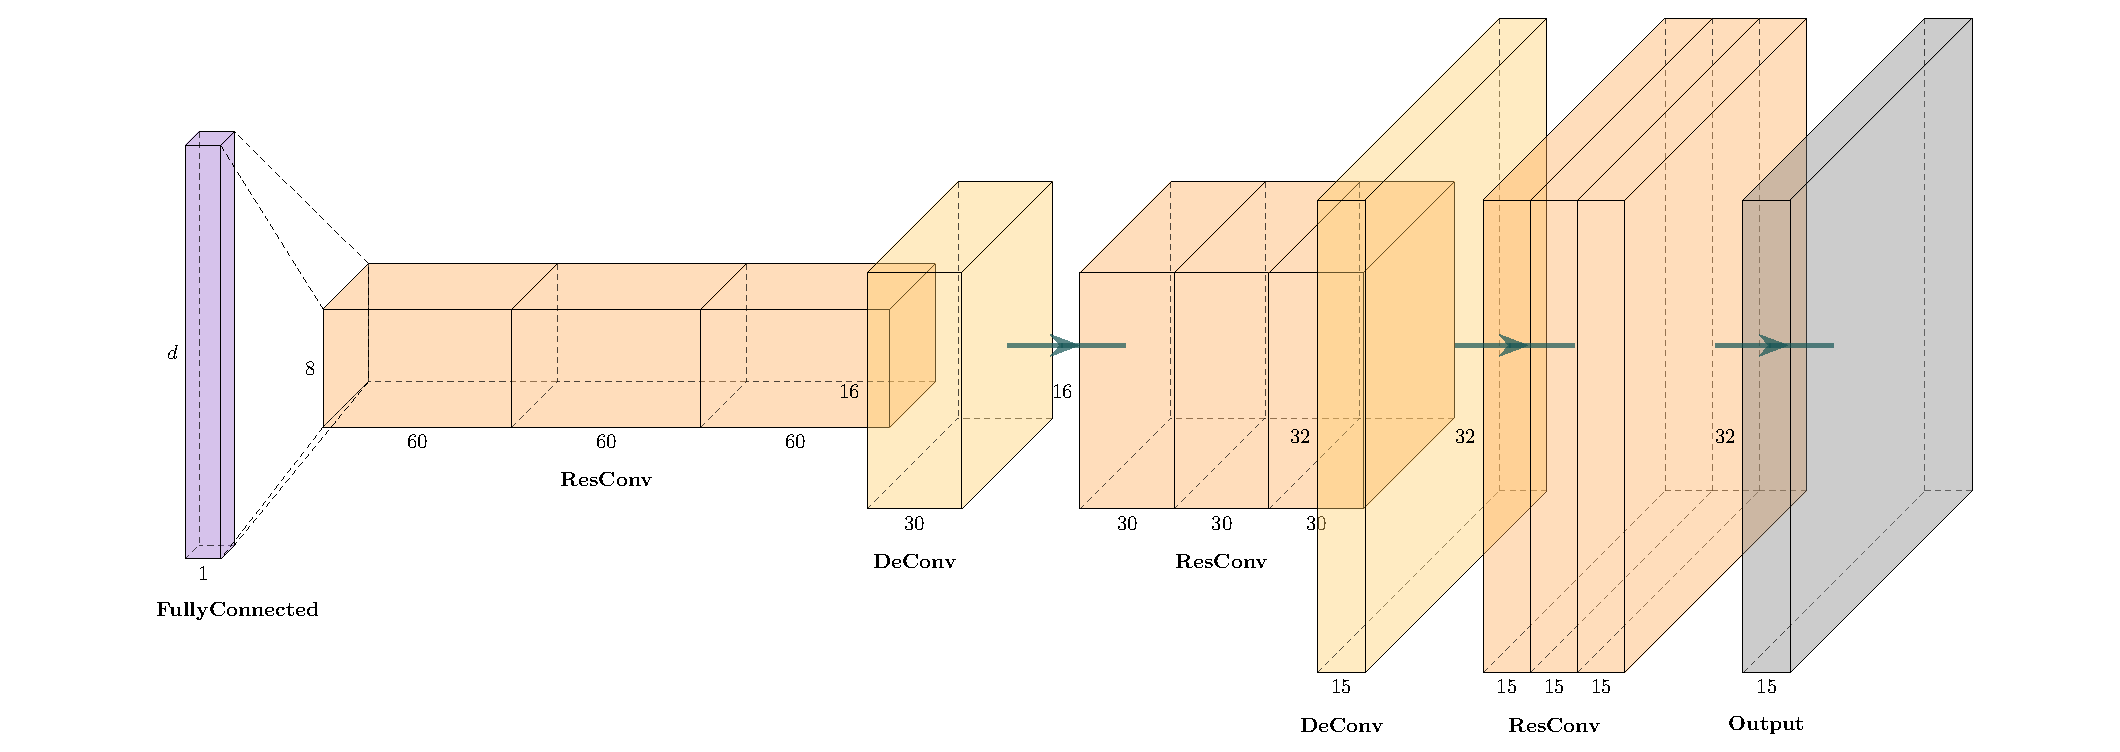
\includegraphics[width=\textwidth]{figures/model_architecture/build/final_vae_decoder.pdf}
        \caption{Final VAE Decoder Architecture (generated with \parencite{NNVisualization})}
        \label{fig:final_decoder}
    \end{minipage}
\end{figure}

The latent dimension $d$, kept at $d = 256$ for the architecture search, is now parametrizable to investigate the impact $d$.
In fact, for this thesis, different latent dimensions are explored: $d \in \{ 256, 512, 1024, 2048 \}$.
The number of parameters of the model in dependence of $d$ is shown in Table \ref{tab:num_parameters}.

\begin{table}[htb]
    \centering
    \begin{tabular}{|c|c|c|}
        \hline
        \textbf{$d$} & \textbf{Encoder Parameters} & \textbf{Decoder Parameters} \\
        \hline
        \hline
        $256$ & 2.2 M & 1.3 M \\
        $512$ & 4.2 M & 2.2 M \\
        $1024$ & 8.1 M & 4.2 M \\
        $2048$ & 16.0 M & 8.1 M \\
        \hline
    \end{tabular}
    \caption{Number of Encoder / Decoder Parameters in Dependence of Latent Dimension $d$}
    \label{tab:num_parameters}
\end{table}

The models are trained on both the complete dataset for $100$ epochs.
The dataset split is $t = 0.13$ and $v = 0.15$, resulting in $13$ cities in the test, $15$ cities in the validation, and $74$ cities in the training set.
The weights of the model with the highest validation \gls{SSIM} during the $100$ epochs is stored.
All other relevant hyperparamaters are kept the same as in Section \ref{section:architecture_search}.

\section{Fine-tuning}
Fine-tuning is a widely adopted technique in machine learning to adapt a base model to a more specific task or dataset \parencite{FineTuning}.
In the context of this thesis, fine-tuning the base \gls{VAE} model to specific cities can enhance the accuracy of emission field reconstructions for those locations.
By tailoring the generative model to the unique characteristics of a city's emission patterns, the model can better capture city-specific structures and variations, improving reconstruction performance based on observed data.

The core idea behind fine-tuning the \gls{VAE} for specific cities is to adjust the range of the generator $G$, which represents the set of all emission fields that the decoder of the \gls{VAE} can generate.
If the emission field to be reconstructed lies outside the generator's range, the model may incur a high representational error, leading to poor reconstruction quality.
By fine-tuning, we effectively modify the generator's range to encompass or closely approximate the target emission fields of the specific cities.

For the fine-tuning experiments, we chose the three cities, Munich, Paris, and Zurich, selected for the case studies.
The fine-tuning process involves updating the weights of the base \gls{VAE} model using city-specific data while employing a reduced learning rate to prevent drastic changes to the model's parameters.
Specifically, we use a learning rate of $10^{-5}$.

The $2015$ emission inventory data is utilized for fine-tuning the model, while the $2018$ data serves as the evaluation dataset to assess the model's performance on updated emission patterns.
Emission fields are cropped at the center, ensuring the model learns the most relevant spatial features.
Besides the temporal scaling factors, random scaling factors are applied to the individual sectors of the emission fields to simulate uncertainties in emission inventories and enhance the model's robustness.
The scaling factors are sampled from the uniform distribution $\mathcal{U}(0.5, 1.5)$, varying the emission intensities by up to $\pm50\%$.
Gaussian noise is added to the emission fields to account for other uncertainties.

Models are fine-tuned for $30$ epochs for each city, sufficient to achieve convergence in the reconstruction errors.
By fine-tuning the \gls{VAE} models to specific cities, we aim to improve the representational capacity of the generator for those cities, thereby enhancing the overall performance of the compressed sensing tasks in the subsequent case studies.
